\chapter{\selectlanguage{greek}Μεθοδολογία}
Στο κεφάλαιο αυτό περιγράφετεαι η προσέγγιση μας στην παραγωγή κώδικα χρησιμοποιώτας αναδραστικά νευρωνικά δίκτυα.
Εμπνεόμαστε απο το blog post του \en{Andrej Karpathy}, στο οπoίο χρησιμοποιείται μια σχετικά απλή δομή RNN με LSTM στοιχεία η οποία εκπαιδεύεται στα έργα του Shakespeare, κατά χαρακτήρα, και παράγει παρόμοιο κείμενο.
Χρησιμοποιούμε το ίδιο μοντέλο, εκπαιδευμενο σε κώδικα \en{javascript}.
Με σκοπό να βελτιώσουμε τις επιδόσεις πρόβλεψης του μοντέλου και να εξετάσουμε τη διαίσθηση οτι με περισσότερη χρήσιμη πληροφορία ο παραγώμενος κώδικας θα είναι ποιοτικότερος, προτείνουμε μία επέκταση του προηγούμενου μοντέλου που χρησιμοποιεί \en{a priori} γνώση για τον κώδικα.
Εξετάζουμε τα μοντέλα σε 2 διαφορετικά σετ δεδομένων.
Παρακάτω ακολουθεί αναλυτική παρουσίαση της μεθόδου.

\section{Τα μοντέλα}

\subsection{\en{Recurrent Neural Networks as Generative Models}}
Ο στόχος της μοντελοποίησης γλώσσας κατα χαρακτήρα (χωρίς να αναφερόμαστε απαραίτητα στην προγραμματιστική γλώσσα) είναι να προβλέψει τον επόμενο χαρακτήρα σε μία ακολουθία.
Δεδομένης μιας εκπαιδευτικής ακολουθίας $(x_1, x_2, ..., x_T)$, τα αναδραστικά νευρωνικά δίκτυα
χρησιμοποιούν τις εξόδους τους $(ο_1, ο_2, ..., ο_T)$ για να πάρουν κατανομές πρόβλέψεων της μορφής $P(x_{t+1}|x_{\leq{t}}) = P(softmax(o_t))$, όπου η κατανομή <<\en{softmax}>> ορίζεται: $P(softmax(o_t) = j) = exp(o_t^{(j)}/\sum_k exp(o_t^{(k)})$.
Ο στόχος που χρησιμοποιείται για την μοντελοποίηση της γλώσσας είναι η μεγιστοποίηση της λογαριθμικής πιθανότητας της εκπαιδευτικής ακολουθίας $\sum_{t=0}^{T-1}logP(x_{t+1}|x_{\leq{t}})$.
Όπως και στην εργασία των Graves et al. \cite{Graves2013}, εισάγουμε στοχαστικότητα δειγματοληπτώντας απο την έξοδο του νευρωνικού δικτύου και δίνοντας την τυχαία επιλογή μας ως είσοδο, την επόμενη χρονική στιγμή.

\subsection{\en{Model char-rnn}}

Το πρώτο μοντέλο είναι ένα αναδραστικό νευρωνικό δίκτυο με 3 κρυμμένα επίπεδα στοιχείων \en{LSTM}.
Δέχεται ακολουθιές χαρακτήρων κώδικα και εξάγει προβλέψεις για τα επόμενα στοιχεία τους.
Η προβλέψεις του char-rnn έχουν μία διάσταση ίση με τον αριθμό διαφορετικών χαρακτήρων που υπάρχουν στο εκάστοτε σετ δεδομένων.   

\begin{figure}[tph]
	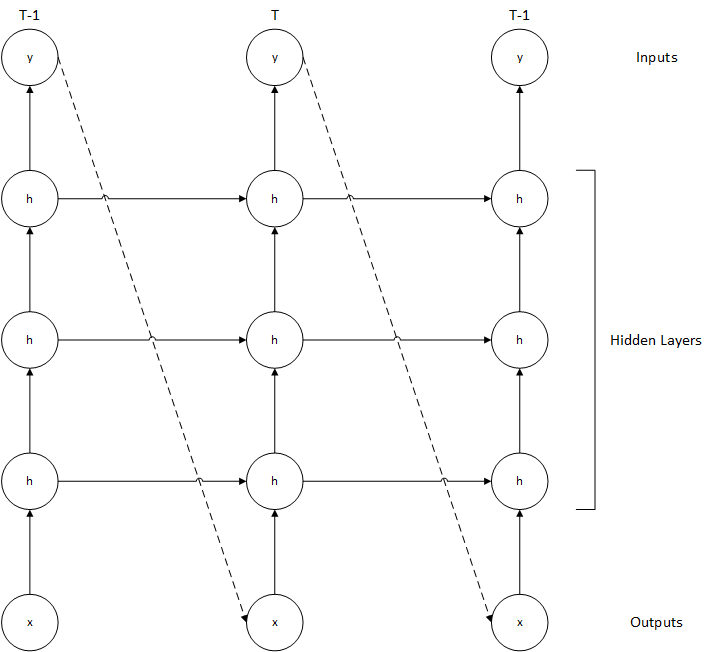
\includegraphics[width=\textwidth, keepaspectratio]{images/char-rnn.png}
	\centering 
	\caption{Το μοντέλο char-rnn.}
	\label{fig:char-rnn}
\end{figure}

\subsection{\en{Model labeled-char-rnn}}

Το δεύτερο μοντέλο είναι επίσης ένα αναδραστικό νευρωνικό δίκτυο με 3 κρυμμένα επίπεδα στοιχείων \en{LSTM}. 
Εκτός απο ακολουθίες χαρακτήρων, το μοντέλο αυτό δέχεται και πληροφορία για το είδος του χαρακτήρα. 
Αντίστοιχα οι έξοδοί του, εκτός απο προβλέψεις για τον χαρακτήρα, περιέχουν και προβλέψεις για το είδος του χαρακτήρα.

\begin{figure}[tph]
	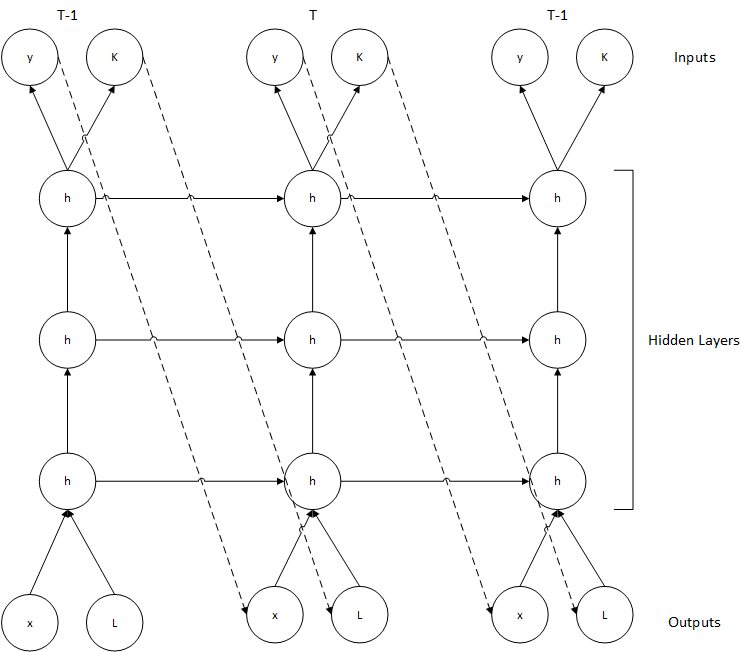
\includegraphics[width=\textwidth, keepaspectratio]{images/l-char-rnn.png}
	\centering 
	\caption{Το μοντέλο labeled-char-rnn.}
	\label{fig:l-char-rnn}
\end{figure}

\section{Τα σετ δεδομένων}

\section{\en{Pre-processing}}

\section{\en{Training}}

\section{\en{Inferring}}
